The results of model independent limits are interpreted in terms of limits
computed for squark pair production with $\squarkprod$ in a SUSY compressed
scenario. The sensitivity to these models is estimated by performing a global
fit that includes the $\crele$, $\crwmn$, $\crzmm$ control regions and all the
systematic uncertainties. The expected limits are derived from the fit procedure
by replacing the data with the background prediction.

Since in the compressed SUSY models the $\met$ recoils typically against several
jets, the average jet momenta are lower than the missing energy, thus requiring
an asymmetric cut on the leading jet momentum and $\met$ to capture this
signal. A signal region (AM1) with $\met > 700$~GeV and leading jet
$\pt > 300$~GeV was defined and compared with the IM1 signal region. The results
for an integrated luminosity of L = 3.2~$\ifb$ for these two signal regions is
presented in Figure~\ref{fig:im1_straight_comparison}, a model is excludable if
the signal strength $\mu$, depicted by the color scale in the picture, is lower
than one. The sensitivity improves for the signal region AM1 to reflect the
asymmetric kinematics.
\begin{figure}[!h]
  \centering
  \begin{subfigure}[t]{.48\linewidth}
    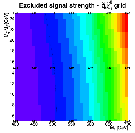
\includegraphics[width=\linewidth]{expected_im1}
    \caption{EM1.}
    \label{fig:expected_im1}
  \end{subfigure}
  \begin{subfigure}[t]{.48\linewidth}
    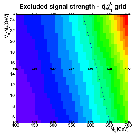
\includegraphics[width=\linewidth]{expected_straight_cut}
    \caption{AM1.}
    \label{fig:expected_straight}
  \end{subfigure}
  \caption{Sensitivity to the compressed SUSY models with an integrated
    luminosity of L=3.3\ifb ~in the plane defined by the squark mass
    $m_{\tilde{q}}$ and the mass difference between the squark mass and the
    lightest neutralino mass
    $\Delta m = m(\tilde{q}) - m(\tilde{\chi}_{1}^{0})$. The color scale
    reflects the lowest excludable signal strength for a particular mass
    point. The values indicated on the map indicate the actual excludable $\mu$
    values at a some specific SUSY models. The dashed line shows the limit
    between excludable and not excludable models. The theoretical uncertainties
    in the signal are not included.}
  \label{fig:im1_straight_comparison}
\end{figure}
In the AM1 signal region, models with mass gaps $\Delta m = 5$~GeV between the
squark mass and the neutralino mass, can be excluded up to squark masses of
650~GeV. At a larger mass gap of $\Delta m = 25$~GeV, squark masses up to
580~GeV are excludable.

The performance of the shape fit method were also tested on the SUSY compressed
spectra; a comparison with the AM1 signal region, is shown in
Figure~\ref{fig:shape_straight_comparison}, the shape fit method improves the
expected limits especially for the largest mass gap of $\Delta m = 25$~GeV
between the squark and the neutralino masses, the AM1 region was thus dropped.
\begin{figure}[!h]
  \centering
  \begin{subfigure}[t]{.48\linewidth}
    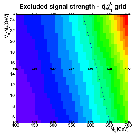
\includegraphics[width=\linewidth]{expected_straight_cut}
    \caption{AM1.}
    \label{fig:expected_im1}
  \end{subfigure}
  \begin{subfigure}[t]{.48\linewidth}
    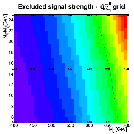
\includegraphics[width=\linewidth]{expected_shape_fit}
    \caption{Shape fit.}
    \label{fig:expected_straight}
  \end{subfigure}
  \caption{Comparison between the results obtained with a straight cut on the
    AM1 signal region and the limits calculated with the shape fit. The
    theoretical uncertainties in the signal are not included.}
  \label{fig:shape_straight_comparison}
\end{figure}

Figure~\ref{fig:expected_observed} shows the result limits on the SUSY
compressed models for the Run~2 2015 data. This is the result of the shape fit
with a luminosity of $3.2~\ifb$ with all theoretical signal systematic
uncertainties included and using the $\crele$, $\crwmn$, $\crzmm$ control
regions. Models with a mass gap of $\Delta m = 5$~GeV between the squark and the
neutralino mass can be excluded up to squark masses of 608~GeV. For larger mass
gap of $\Delta m = 25$~GeV, squark masses up to 532~GeV are also excluded.
\begin{figure}[!h]
  \centering
    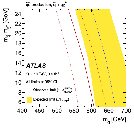
\includegraphics[width=.5\linewidth]{expected_observed}
    \caption{Expected and observed limits on the SUSY compressed models using
      the Run~2 2015 data, in the plane defined by the squark mass on the
      $x$-axis and the mass difference between the squark and lightest
      neutralino mass on the $y$-axis. All experimental and theoretical
      systematic uncertainties are included.}
\label{fig:results:susy:compressed_observed}
    \label{fig:expected_observed}
\end{figure}
%%% Local Variables:
%%% mode: latex
%%% TeX-master: "../search_for_DM_LED_with_ATLAS"
%%% End:
